\begin{exercise}
Betrachten Sie für $r \in \R$ die autonome ODE
\begin{align*}
  y^{\prime} = y + \tanh(ry).
\end{align*}
Wieviele Ruhelagen hat die Gleichung abhängig von $r$? Um welchem Typ von Bifurkation
handelt es sich beim Bifurkationspunkt $r = 1$?
\end{exercise}
\begin{solution}
Bestimmen wir zuerst die Ruhelagen der ODE:
Für alle $r$ sehen wir aufgrund $\tanh(0) = 0$, dass $y^* = 0$ eine Ruhelage der ODE
sein muss.
Die Nullstellen direkt zu berechnen sieht eher schwierig aus, daher betrachten wir
einmal die Extremwerte.
\begin{align*}
  f^{\prime}(y) = 1 + r(1 - \tanh(ry)^2) = 1 + r - r\tanh(ry)^2.
\end{align*}
Fall 1: $r \geq 0:$
\begin{align*}
  f^{\prime}(y) \geq 1
\end{align*}
Fall 2: $-1 < r < 0$:
\begin{align*}
  f^{\prime}(y) > -r\tanh(ry)^2 \geq 0
\end{align*}
Fall 3: $r = -1$:
\begin{align*}
  f^{\prime}(y) &\geq 0 \\
  f^{\prime}(0) &= 0.
\end{align*}
In allen Fällen ist die Funktion also streng monoton steigend und kann damit
nur die Nullstelle $y^* = 0$ besitzen. \\
Fall 4: $r < -1$:
\begin{align*}
  f^{\prime}(0) &= 1 + r - r\tanh(0)^2 = 1 + r < 0 \\
  \lim_{y \to \pm\infty}f^{\prime}(y) &= 1 + r - r = 1 > 0 \\
\end{align*}
Also ist $f$ in einer Umgebung von $0$ streng monton fallend und es exisitieren
$y_0 > 0: f(y_0) < 0$ und $y_1 < 0: f(y_1) > 0$. Gleichzeitig gilt
\begin{align*}
  \lim_{y \to \infty} f(y) &= \infty \\
  \lim_{y \to -\infty} f(y) & -\infty.
\end{align*}
Laut dem Zwischenwertsatz hat $f$ für $r < -1$ also mindestens drei Nullstellen.
Seien $y_-^*,y_+^*$ die erste negative, beziehungsweise positive Nullstelle von $f$.
Dann folgt für $y > y_+^*$ aufgrund der Monotonie des Tangens Hyperbolicus:
\begin{align*}
  f(y) = y + \tanh(ry) > y_+^* + \tanh(ty_+^*) = 0.
\end{align*}
Analog folgt für $y < y_-^*: f(y) < 0$. Also kann $f$ nur genau diese drei Nullstellen haben. \\
Der Bifurkationspunkt ist also $r = -1$, in welchem aus einer Ruhelage 3 Ruhelagen werden.
Das nennt man auch \glqq supercritical pitchfork bifurcation \grqq. \\
Jetzt kann man noch die Stabilität der Ruhelagen untersuchen, bin mir aber
nicht sicher, ob das gefordert ist.
\FloatBarrier
\begin{figure}
    \centering
    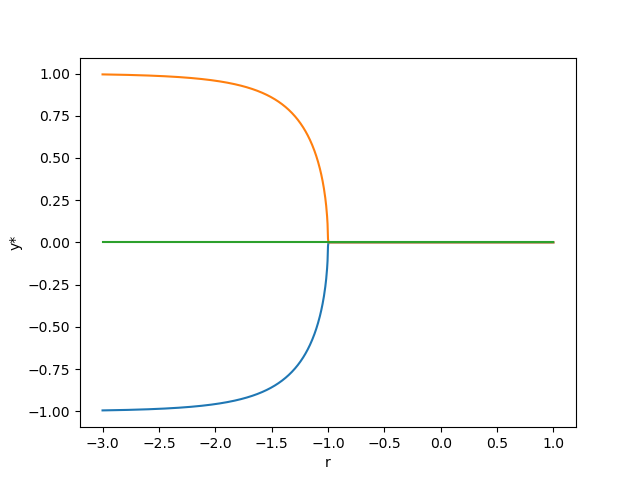
\includegraphics[width=\linewidth]{bifurcation_plot.png}
    \caption{Ruhelagen in Abhängigkeit von $r$}
\end{figure}
\FloatBarrier
\end{solution}
